\chapter{Critical Success Factor Analysis Based on Feature Selection}
\label{apx:b_csf_fs}


Critical Success Factor (CSF) is a management term for an element that is necessary for an organization or project to achieve its mission. CSFs represent the principal assets or areas that must be given investments to achieve better results. CSF analysis is one challenger strategic management tool, which can provide a robust and very practical assessment for strategic planners.

The identification of the most significant information for one problem is referred to as feature selection by the signal processing and data mining areas, as well as it can be formulated as a principal component problem, which is a widely adopted signal processing technique for data visualization and feature extraction. Feature selection aims to select a subset of relevant information from a larger dataset, in order to improve: data visualization and data understanding, storage requirements, dimensionality, processing time, discriminative sensing, and to overcome overfitting problems to improve prediction and classification performance \cite{chandrashekar2014survey}.

Recursive Feature Elimination (RFE) is a feature selection method for small sample classification problems. RFE seeks to improve generalization performance by recursively removing the least significant features whose deletion will have the least effect on training errors, according to the higher variance measured from the features \cite{chen2007enhanced}.

We propose a critical factors analysis based on Principal Component Analysis (PCA) for visual discriminant analysis and based on RFE combined with Support Vector Machine (SVM) \cite{hearst1998support}, applied to the survey that evaluates the IT governance of Brazilian public organizations, in order to identify the CSF for IT governance of the public sector according to TCU. Results show how PCA can make the data discriminative and that SVM is the classifier that best performs and obtains an accuracy of 91.42\% to learn and classify according to TCU's IT governance evaluation of Brazilian public sector. Finally, SVM is used to highlight the more significant features identified by RFE, which are similar to CSFs previously identified by a qualitative analysis of the same dataset.

This chapter is organized as follows. In Section \ref{sec:b_relatedworks}, related works are discussed. Section \ref{sec:b_datamodel} presents the data model and the evaluated datasets. Section \ref{sec:b_csf_fs} describes the proposed approach for critical success factors analysis. Section \ref{sec:b_experimentalresults} discusses the experimental validation and presents the results, and Section \ref{sec:b_conclusion} draws the conclusions.


\section{Related Works}
\label{sec:b_relatedworks}

Fink and Sukenik \cite{fink2011effect} explore the relationships among IT infrastructure capability and IT business value using PCA applied to all indicators of their study, resulting into 11 factors, with the first factor accounting for only 27.9\% of the variance. This technique was used because the PCA extracts orthogonal factors that overcome the problem of multicollinearity.

Ramos \emph{et al} \cite{ramos2016information} propose an overview regarding the evolution of scientific research on IT Governance critical success factors within the domain of public administration. By means of bibliometric analysis it was investigated seminal works regarding this theme, considering the characteristic key words found during our analysis. The results present 64 critical success factors with high impact on IT governance.

Guyon \emph{et al} \cite{guyon2002gene} propose a method of gene selection utilizing Support Vector Machine methods based on Recursive Feature Elimination (RFE) and demonstrate that the selected genes yield better classification performance and are biologically relevant to cancer.  The proposed method eliminates gene redundancy automatically and yields better and more compact gene subsets. 

To the best of our knowledge, we are the first to propose a critical factors analysis based on PCA for visual discriminant analysis and based on RFE combined with SVM for CSF identification from IT governance data.


\section{Data Model}
\label{sec:b_datamodel}

The Brazilian Federal Court of Accounts (TCU, in Portuguese) surveys data regarding IT practices of Brazilian public organizations in order to audit IT governance. The dataset with a consolidate view about the answers for this survey the IT governance index is called iGovTI. The iGovTI is composed by 201 multiple choice questions, used for ranking according to their IT governance, submitted to 349 organizations. The TCU computes the IT governance index and classifies the IT governance of each organization. Additionally, Ramos \emph{et al} \cite{ramos2016information} classifies each question regarding its relevance for IT governance through a qualitative analysis, and identify the CSFs for selected IT managers regarding IT governance.


\section{An approach for Critical Success Factors Analysis}
\label{sec:b_csf_fs}

In this section we propose an approach for CSF Analysis based on visual discriminant analysis and based on feature selection, in order to identify the CSFs for IT governance according to iGovTI. Initially we conduct an analysis based on PCA to evaluate the relevance of each question according to their variance, and use the 2 most relevant features for a visualization of the iGovTI ranking. Furthermore, we propose a critical success factors analysis based on SVM for classification and based on RFE for identification of the most relevant factors.

\subsection{Visual Discriminant Analysis based on PCA}
\label{sec:b_pca}

PCA is a statistical technique commonly used for signal denoising, blind source separation, data compression, data visualization, feature extraction and dimensionality reduction, where a reduced number of features is extracted retaining as much information as possible \cite{jolliffe1986principal}. It uses an orthogonal transformation to convert a set of correlated variables into a set of linearly uncorrelated variables, where the first principal components have the largest variance.

PCA is an orthogonal basis transformation into new basis, by diagonalizing the centered covariance matrix of a data set \{$\mathbf{x}_j \in \mathbb{R}^m, j = 1, ... ,n$\}, defined by $\mathbf{C} = \frac{\mathbf{X}^\intercal\mathbf{X}}{n}$, where $\mathbf{X} = (\mathbf{x}_1, ... , \mathbf{x}_n)^\intercal$ and the samples are assumed to have zero mean. The eigenvectors $\mathbf{v}_i$ of $\mathbf{C}$ are called principal components (PC), and the sample variance along $\mathbf{v}_i$ of $\mathbf{C}$ is given by the corresponding eigenvalue $\lambda_i$. Projecting onto the eigenvectors with the largest eigenvalues assumes that minimal information is lost, considering that in many applications these directions contain the most interesting information, such as in in data compression and denoising.

Initially, we compute the covariance matrix $\mathbf{C}$ of a zero mean data and visualize the data relationship for the sample covariance. Sample covariance is calculated by computing deviations of each measurement from the average of all measurements for that variable. Then the deviations for the two measurements are multiplied together separately for each subject. Finally these values are averaged. After that, the eigenvectors $\mathbf{v}_i$ and eigenvalues $\lambda_i$ of $\mathbf{C}$ are computed through Singular Value Decomposition (SVD), then it is possible to evaluate the variance distribution of the extracted components through an empirical cumulative distribution function (ECDF). Evaluating the variance distribution we expect to visualize if some features concentrates the variance and indicates advantages for dimensionality reduction.

Finally, we propose to select the two features with the largest variance and evaluate the relationship between the two principal components and the iGovTI classification, in order to visualize if there is a segmentation according to the iGovTI ranking.

Considering that PCA combines attributes and creates new ones, with measurements from all of the original variables, it is hard to identify what original variables are most relevant. Therefore, it is still necessary an additional method to reveal what are the CSF for iGovTI. For this problem, we propose a CSF analysis based on RFE.

\subsection{CSF analysis based on RFE}
\label{sec:b_csfa}

Feature selection aims the identification of the most significant information for one problem or algorithm, such as classification or prediction problems. RFE is a feature selection method for small sample classification problems by recursively removing the least significant features whose deletion will have the least effect on training errors, according to the higher variance measured from the features through a selected classifier. 

Initially, it is necessary to identify one classifier that can identify the iGovTI classification of one organization according to a training dataset. Therefore, we propose an algorithm evaluation in order to identify which one presents the best accuracy for iGovTI classification. The selected algorithm should be used by RFE to identify the CSF, that should be compared to results of the CSF qualitative analysis conducted by Ramos \emph{et al} \cite{ramos2016information}.

Feature selection doesn't combine attributes, as PCA, but just evaluates their informative quality, predictive power and select the best set. Given an external estimator or classifier, that assigns weights to features, RFE is able to select features by recursively considering smaller and smaller sets of features. First, the estimator is trained on the initial set of features and the importance of each feature is obtained either through a coefficient attribute or through a feature importances attribute. Then, the least important features are pruned from current set of features. That procedure is recursively repeated on the pruned set until the desired number of features to select is eventually reached. RFE can also rank all features according to when they were eliminated. 

The variables with the least effect on training errors or largest weights indicates more relevance for a classifier. Therefore, we propose to assume that the selected most relevant features are the CSF for iGovTI and also propose to validate this assumption against the results of the CSF qualitative analysis conducted by Ramos \emph{et al} \cite{ramos2016information}.


\section{Experiments and Results}
\label{sec:b_experimentalresults}

In this section we present the experiments and results for the visual discriminant analysis based on PCA and for CSF analysis based on RFE, and discuss the results.

For the visual discriminant analysis we initially we compute the zero mean and the the covariance matrix $\mathbf{C}$ is computed from $\mathbf{X}$.The results are shown by Figure \ref{fig:ch2_fig1}.
 
\begin{figure}[h!]
     \centering 
     \includegraphics[height=10cm, width=10cm]{figures/ch2/raw_igovti_covariance.eps}
     \caption{Covariance matrix of iGovTI questions.}
     \label{fig:ch2_fig1}
\end{figure}

Figure \ref{fig:ch2_fig1} presents the covariance matrix of 201 questions of iGovTI, where is possible to observe low covariance for the majority questions and high variance for just a few questions. 

In the next step the eigenvectors $\mathbf{v}_i$ and eigenvalues $\lambda_i$ of $\mathbf{C}$ are computed through SVD. Considering that the first principal components have the largest variance indicated by their eigenvalues, it is necessary to evaluate the variance distribution of the measured eigenvalues. Therefore, we present the Figure \ref{fig:ch2_fig2}, wich shows the variance ECDF of the iGovTI questions and shows that 97\% of the questions have variance lesser than 2, while just 3\% of the questions have variance between 2 and 11. This result indicates that just a few principal components concentrates the most significant information and motivates the evaluation regarding the relationship between the principal components and the iGovTI classification.

\begin{figure}[h!]
     \centering 
     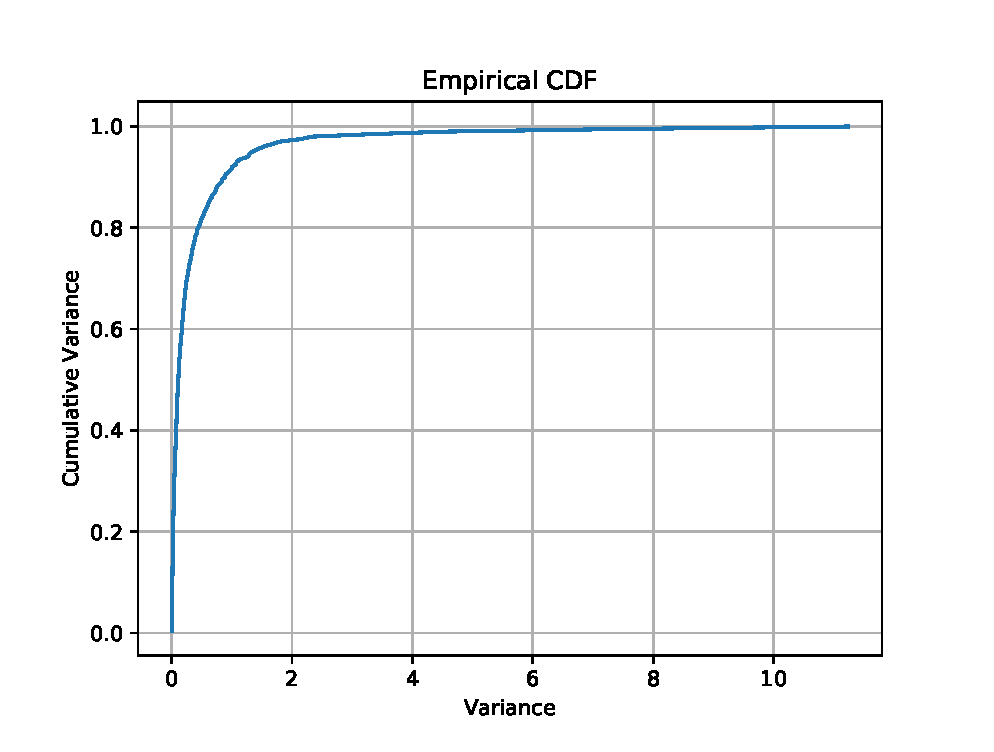
\includegraphics[height=8cm, width=11cm]{figures/ch2/raw_variance_ecdf.eps}
     \caption{Empirical CDF of variance.}
     \label{fig:ch2_fig2}
\end{figure}
 
Finally, we select the two largest eigenvalues and their correspondent components in order to evaluate the relationship between the iGovTI classification for 349 organizations and the two most informative variables. The Figure \ref{fig:ch2_fig3} shows the scatter diagram that plots the organizations with higher iGovTI with larger circumferences and colors near of red, while organizations with lower iGovTI have colors near of blue and shorter circumferences. It is possible to observe that organizations with higher iGovTI are concentrated in the top left quadrant, with a visual separation of organizations with lower iGovTI, but without a clear distance separating the classes.
 
\begin{figure}[h!]
     \centering 
     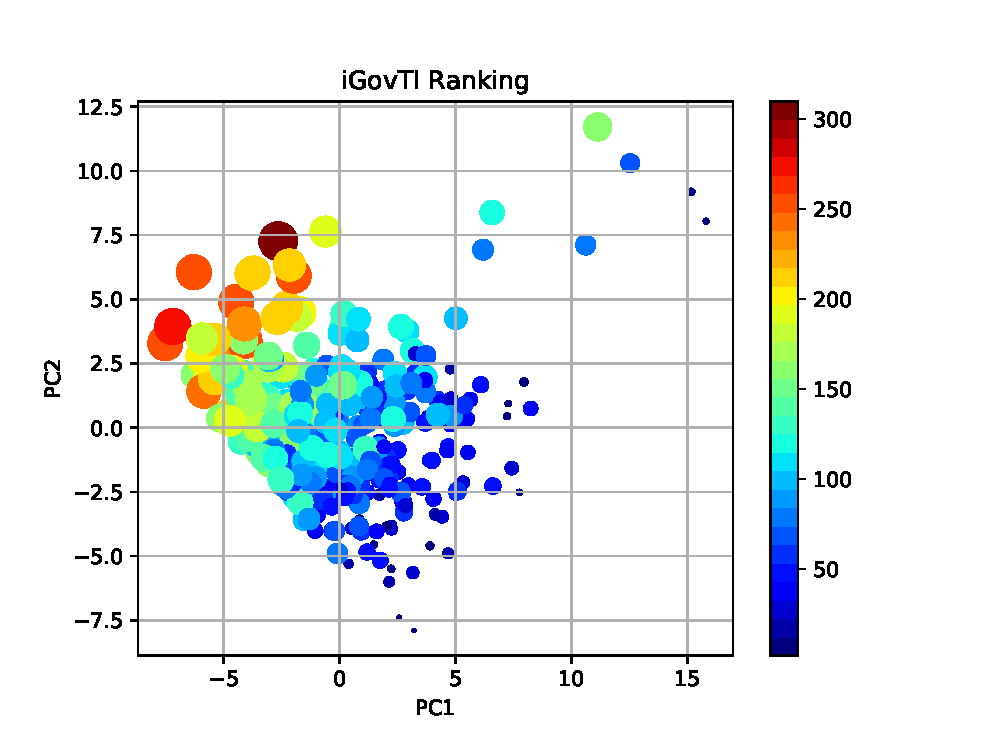
\includegraphics[height=8cm, width=11cm]{figures/ch2/raw_igovti_ranking_pc2.eps}
     \caption{iGovTI ranking from 2 principal components.}
     \label{fig:ch2_fig3}
\end{figure}

The visual discriminant analysis indicates that just a few principal components concentrates the most significant information and that the two principal components show a visual classification of organizations according to iGovTI classification, however it is not clear what are the CSF. 

Hence, it is necessary additional techniques for CSF identification and we propose a critical success factors analysis based on RFE for identification of the most relevant factors for iGovTI.

RFE requires a classifier or predictor to evaluate its generalization performance by recursively removing the least significant features whose deletion will have the least effect on training errors, according to the higher variance measured from the features. We perform an algorithm evaluation in order to identify the classifier with the highest accuracy for iGovTI classification. The evaluated dataset is composed of 201 questions (features) and 349 organizations (observations), where each organization is classified according to iGovTI classes, which are initial, intermediate and enhanced. We divide the dataset into train and test, with the training data equivalent to 90\% of the whole dataset, while the test has 10 \% of the whole dataset.

The Table \ref{tab:ch2_tab1} present the selected classification algorithms and the measured accuracy for iGovTI classification. According to results, SVM \cite{hearst1998support} is the algorithm with highest classification accuracy, with 91.42\%, while the second is Elastic Net \cite{zou2005regularization}, with 83.15\% of accuracy. The results for iGovTI classification corroborates previous evaluations that highlight the advantages of SVM for classifications from small datasets \cite{guyon2002gene}. Additionally, our results indicate that SVM is the best classifier for RFE, which corroborates the previous research of Guyon \emph{et al} \cite{guyon2002gene}, where is proposed SVM-RFE, that is a method of gene selection utilizing SVM methods based on RFE. 	

\begin{table*}[!t]
	\caption{Evaluation of classification accuracy for iGovTI}
  	\label{tab:ch2_tab1}
	\centering
	\begin{tabular}{|l|r|}
		\hline \rowcolor{Gray} Algorithm	& Mean Accuracy\\\hline
		Linear Regression \cite{draper2014applied}	&0.3608\\ \hline
		LDA \cite{martinez2001pca}	&0.6285\\ \hline
		K-Nearest Neighbors \cite{fukunaga1975branch}	&0.7142\\ \hline
		Linear SVM \cite{fan2008liblinear}	&0.7142\\ \hline
		Logistic Regression \cite{hosmer2013applied}	&0.7714\\ \hline
		SVM Regression \cite{smola2004tutorial}	&0.8268\\ \hline
		Lasso \cite{tibshirani1996regression}	&0.8274\\ \hline
		Elastic Net \cite{zou2005regularization}	&0.8315\\ \hline
		SVM \cite{hearst1998support}	&0.9142\\ \hline
	\end{tabular}
\end{table*}

The next step is to use the selected algorithm as validator for recursive feature elimination in order to identify the CSF for iGovTI. Additionally, the RFE algorithm requires the number of desired most significants features. We adopt 54 for this variable, considering that is the number of CSF identified by Ramos \emph{et al} \cite{ramos2016information} in a qualitative analysis, that is the proposed target to validate the results of the CSF identification for iGovTI.

The RFE algorithm presents an ranking according to the significance of each feature, with an accuracy of 69,9\% for CSF classification when compared to the CSF identified by Ramos \emph{et al} \cite{ramos2016information} in a qualitative analysis.


\section{Conclusion}
\label{sec:b_conclusion}

The proposed approach is evaluated and the experimental results show that the visual discriminant analysis, through PCA, highlights important characteristics of the data, and that a selected classifier and RFE can be applied for iGovTI classification and for CSF identification. 

Results show how PCA can make the data discriminative, however it is hard to identify what original variables are most relevant. Therefore, it is still necessary an additional method to reveal what are the CSF for iGovTI. For this problem, we propose a CSF analysis based on RFE. Since RFE depends on a classifier to select the most relevant features, we perform an algorithm evaluation to identify the classifier with the highest performance, and results show that SVM \cite{hearst1998support} presents the best accuracy, with 91.42\%. 

Finally, SVM is used to select the more significant features identified by RFE, which are 69,9\% similar to CSFs previously identified by a qualitative analysis of the same dataset.